\documentclass[a4paper, 12pt]{article}

\setlength\parindent{0pt}
\usepackage{geometry}
\usepackage{graphicx}
\usepackage{fancyhdr}
\usepackage{minitoc}
\usepackage{enumitem}
\usepackage{wrapfig}
\usepackage[font=small]{caption}
\usepackage{setspace}
\usepackage{hyperref}% add hypertext capabilities
\hypersetup{
    colorlinks=true,
    linkcolor=blue,
    filecolor=magenta,      
    urlcolor=black,
    citecolor=blue,
}
\usepackage{xcolor}

% \usepackage[
%     backend=biber,
%     style=phys,
%     giveninits,
%     minbibnames = 2,
%     maxbibnames=3,
% ]{biblatex}

\usepackage[square, numbers, sort&compress]{natbib}
\bibliographystyle{apsrev4-1}
%\usepackage{doi}%<----------


%\DeclareFieldFormat{labelnumberwidth}{\mkbibbrackets{#1} }
%\addbibresource{bibliography.bib}
% Configure page margins with geometry

\geometry{left=1in, top=1in, right=1in, bottom=1.2in, footskip=1.3cm}
\linespread{1.05}
\renewcommand*{\bibfont}{\small}

%%%%%%%%%%%%%%%%%% new commands %%%%%%%%%%%%%%%%%%%%%
\colorlet{lighttext}{black}

\newcommand*{\footerstyle}[1]{{\fontsize{10pt}{1em}\scshape\color{lighttext} #1}}

\newcommand*{\makecvfooter}[3]{%
  \fancyfoot{}
  \fancyfoot[L]{\footerstyle{#1}}
  \fancyfoot[C]{\footerstyle{#2}}
  \fancyfoot[R]{\footerstyle{#3}}
}

\renewcommand{\headrulewidth}{0pt}

%%%%%%%%%%  footer and title %%%%%%%%%%%%
%\title{\raggedright \huge Exploring unconventional superconductivity through synchrotron and deep~--~learning techniques}
%\date{\vspace{-10ex}}

%%%%%%%%%%%%%%%%%%%%%%%%%%%%%%%%%%%%%%%%%%%%%%%%%%%%%%%%%

\begin{document}
{\huge Exploring unconventional superconductivity \\ through synchrotron and deep learning \\ techniques}
\vspace{0.15cm}
%%%% makes the header and footer %%%%
%\maketitle

%%%%%%%% created the footer %%%%%%%%
\pagestyle{fancy}
\fancyhf{} % sets both header and footer to nothing
\makecvfooter
  {January 2023}
  {\centering Leonardo Martinelli ~~~·~~~ Research Project}
  {\thepage}
%\noindent{\huge UZH PostDoc Grant -  Research proposal}

\vspace{0.3cm}
{\Large Leonardo Martinelli}

\vspace{0.2cm}

{\Large UZH PostDoc Grant - Research proposal}

%\vspace{0.1cm}

%\tableofcontents
%\minitoc
\bigskip 

% \begin{abstract}
% \noindent The driving force behind progress in modern technology is the ability to understand and control materials on a fundamental level. As silicon completely reshaped electronics in the last century, a new revolution is already starting, seeded by another class of materials. Quantum materials are defined as those systems where the microscopic interactions cause the emergence of quantum properties on a macroscopic scale, defying any interpretation in terms of basic solid-state physics. Among the plethora of quantum materials, the most fascinating and promising ones are unquestionably unconventional superconductors. In the last years, they have found applications in medical imaging and high-field magnets, but they are expected to drive disruptive breakthroughs in quantum sensing, energy production and transmission, and quantum computing. However, exploitation of unconventional superconductors requires a complete understanding of the physical mechanisms governing their properties, which is at present largely lacking. This is the goal to which this project aims at contributing. To do that, we will make use of state-of-the-art synchrotron research facilities to investigate the fundamental properties of different classes of superconductors. Additionally, we will push the boundaries of the experimental techniques themselves, by exploring how deep-learning methods can boost the performance of existing instruments. We are confident that our results will produce an immediate impact on the condensed matter physics community, and on technological applications in the long run.
% \end{abstract}

\begin{abstract}
The driving force behind progress in modern technology is the ability to understand and control materials on a fundamental level. As silicon completely reshaped electronics in the last century, a new revolution is already starting, seeded by \emph{quantum materials}. In these systems, the microscopic interactions cause the emergence of quantum properties on a macroscopic scale, defying any interpretation in terms of basic solid-state physics. Among the plethora of quantum materials, the most fascinating and promising ones are unquestionably unconventional superconductors. 
They are expected to drive disruptive breakthroughs in a wide range of applications, ranging from medical sensing to quantum sensing and computing.
However, exploitation of unconventional superconductors requires a complete understanding of the physical mechanisms governing their properties, which is at present largely lacking. Interestingly, many of the unknown properties are related to the normal state of these materials, above the superconducting temperatures. This is the goal to which this project aims at contributing.  
I will focus on charge-order, a phase with broken translational symmetry whose phenomenology is still largely unexplained. I will investigate its properties in two material families:  high-temperature superconducting cuprates and the newly discovered class of infinite-layer nickelates. 
To do that, I will make use of state-of-the-art synchrotron research facilities, as well as uniaxial pressure cells developed in the group of Prof.~Chang at UZH. 
At the same time, I will push the boundaries of the experimental techniques themselves, by exploring how deep-learning methods can boost the performance of existing instruments. Specifically, I will develop a convolutional neural network with the aim of denoising Resonant Inelastic X-ray Scattering data.
I am confident that my results will produce an immediate impact on the condensed matter physics community, and on technological applications in the long run.
\end{abstract}

\section{Objectives of the project}
This Post-Doctoral project is articulated in three milestones. The first part of the project concerns an innovative development of Resonant Inelastic X-ray Scattering. The other two involve the use of different x-ray techniques for the study of a fundamental phenomena in strongly-correlated systems: charge order. 

\medskip

{\bfseries Milestone 1: Deep learning methods for RIXS denoising.} \newline
Resonant Inelastic X-ray Scattering (RIXS) has become a fundamental tool for the investigation of strongly correlated materials, but is strongly limited by its rather long acquisition times and comparatively short beam time allocation. We propose to tackle this problem from an innovative angle, by applying modern deep learning techniques to filter-out the noise of RIXS measurements and with that reduce acquisition times. Application of algorithms for image denoising to physics and chemistry techniques has been extremely limited \cite{valensise2020removing}.
Only very recently, Professor Chang’s group has explored the implementation of such methods to retrieve weak signals from noisy diffraction measurements \cite{oppliger2022weak}. Along the same line, we will explore how Convolutional Neural Networks (CNN) can denoise signals buried in Poisson noise, using supervised learning on pairs of high-noise and low-noise measured data. 
This will be possible not only thanks to the expertise of Prof.~Chang’s group in machine learning algorithms, but also to the large datasets of RIXS data held by the host and the home institution. Our study would have impact beyond the RIXS technique, and could be applied to similar techniques such as (non-resonant) Inelastic Neutron or X-ray Scattering. We therefore expect our results to have a strong impact on the entire condensed matter physics community.

\medskip

{\bfseries Milestone 2: Coupling of charge order with phonons in strongly-correlated systems.}
Uniaxial pressure application is an important tool for investigation of quantum materials. It has been used in combination with transport, ARPES and diffraction experiments \cite{lin2021visualization, arpaia2019dynamical, wang2022uniaxial}. However, it has not been widely implemented in combination with state-of-the-art RIXS experiments. Here we propose to adapt uniaxial pressure cells – designed and developed by the laboratory – to reach compatibility with the most modern RIXS instruments. With such technical advancement, we will address the important problem of charge order in the context of cuprate high-temperature superconductivity \cite{cubrovic2009string, arpaia2019dynamical}. Its origin is still strongly disputed, and anomalies in recent experiments have been interpreted in terms of both charge excitations \cite{chaix2017dispersive,li2020multiorbital} and phonons \cite{wang2021charge}. In this project, we will address the question using uniaxial strain to de-twin charge-order domains \cite{wang2022uniaxial}, effectively pinning them to a single direction in real space. We will then measure phonon spectra along the two direction (with and without charge-order) using Resonant (RIXS) and non-resonant Inelastic X-ray Scattering (IXS), precisely quantify for the first time the renormalization of the phonon propagator for high- and very-low-energy phonon branches. This experiment will provide fundamental information on the physics of charge order in cuprates, and settle a fifteen years old problem.

\medskip 

{\bfseries Milestone 3: Structure of charge order in Nickelates.}
The recent synthesis of superconducting nickelate films has generated much enthusiasm in the condensed matter community: their electronic and structural similarity to cuprates allows to use them as a benchmark for theories on unconventional superconductivity \cite{li2019superconductivity}. Last year three independent works, one of which I authored, used soft x-ray RIXS to report the presence of charge-order in these compounds, with some significant differences with respect to cuprates \cite{krieger2022charge, rossi2022broken, tam2022charge}. Currently, further progress is held back because only soft x-rays (implying limited reciprocal space) have been applied. Here, we propose to study its three-dimensional structure in reciprocal space using surface diffraction, as a function of temperature and doping. This project is enabled by the P07 beam line at DESY (Hamburg), where cryogenic sample environment is recently made compatible with surface diffraction. 

\medskip

\section{State of research}
Quantum materials are characterized by an emergence of purely quantum mechanical effects on a macroscopic scale, produced by either low-dimensionality, topology, or strong entanglement between the electrons. Among them, unconventional superconductors hold prominent importance, and probably represent the best example of a coherent, macroscopic quantum state. Their astonishing properties led to applications in high-field magnets \cite{weijers2010high}, medical sensing \cite{iwasa2010high} and magnetometry \cite{clarke2004squid}, and more recently in quantum computations \cite{ladd2010quantum}.
The importance of unconventional superconductors is, however, not just limited to technological applications. The description of their microscopic state defies any trivial treatment in terms of basic solid-state physics. 
The superconducting state itself, which for “trivial” BCS-superconductors is described in terms of an isotropic order (s-wave), spin-singlet order parameter, can display more complicated symmetries such as $p$-, $d$-, or even $f$-wave, and even a spin-triplet nature \cite{ran2019nearly}. 
For most of them, the interaction that drives the pairing is still not established, and there are no first-principle calculations which can reproduce the entirety of experimental observations.
The mysterious properties extend, however, to the ``normal'' state above the superconducting transition. 
Most importantly, it displays several anomalous properties which are shared among many families of strongly correlated superconductors: $T$-linear resistivity and peculiar magneto-transport coefficients are observed (among others) in cuprates \cite{cooper2009anomalous, jin2011link, chien1991effect}, iron pnictides \cite{licciardello2019electrical}, ruthenates \cite{bruin2013similarity}, and heavy-fermion materials \cite{lai2022electronic, paschen2004hall}. More recently, they have also been discovered in twisted bilayer graphene, where the correlation between electrons is produced by the emergence of flat bands at the Fermi level \cite{polshyn2019large}.
The universality of such properties, shared between materials with very different structures, chemical composition, and electronic structure probably represents the biggest unsolved question in condensed matter physics \cite{phillips2022stranger}.
Recent theories postulate an entanglement between electrons so deep to constitute a new phase of matter, which possibly carries some similarities with black holes \cite{zaanen2019planckian, zaanen2021lectures, PhysRevD.105.L021901}. Moreover, the architecture of such theories is directly linked to modern string theory \cite{cubrovic2009string}, so that these materials might even provide a benchmark to test the validity of much more fundamental theories.
%Another crucial property of the normal ($T>T_c$) state of these materials indeed displays different types of broken translational and rotational symmetries, which involve either the charge, spin, or orbital degrees of freedom \cite{keimer2015quantum}.
%
\begin{figure}[t]
    \centering
    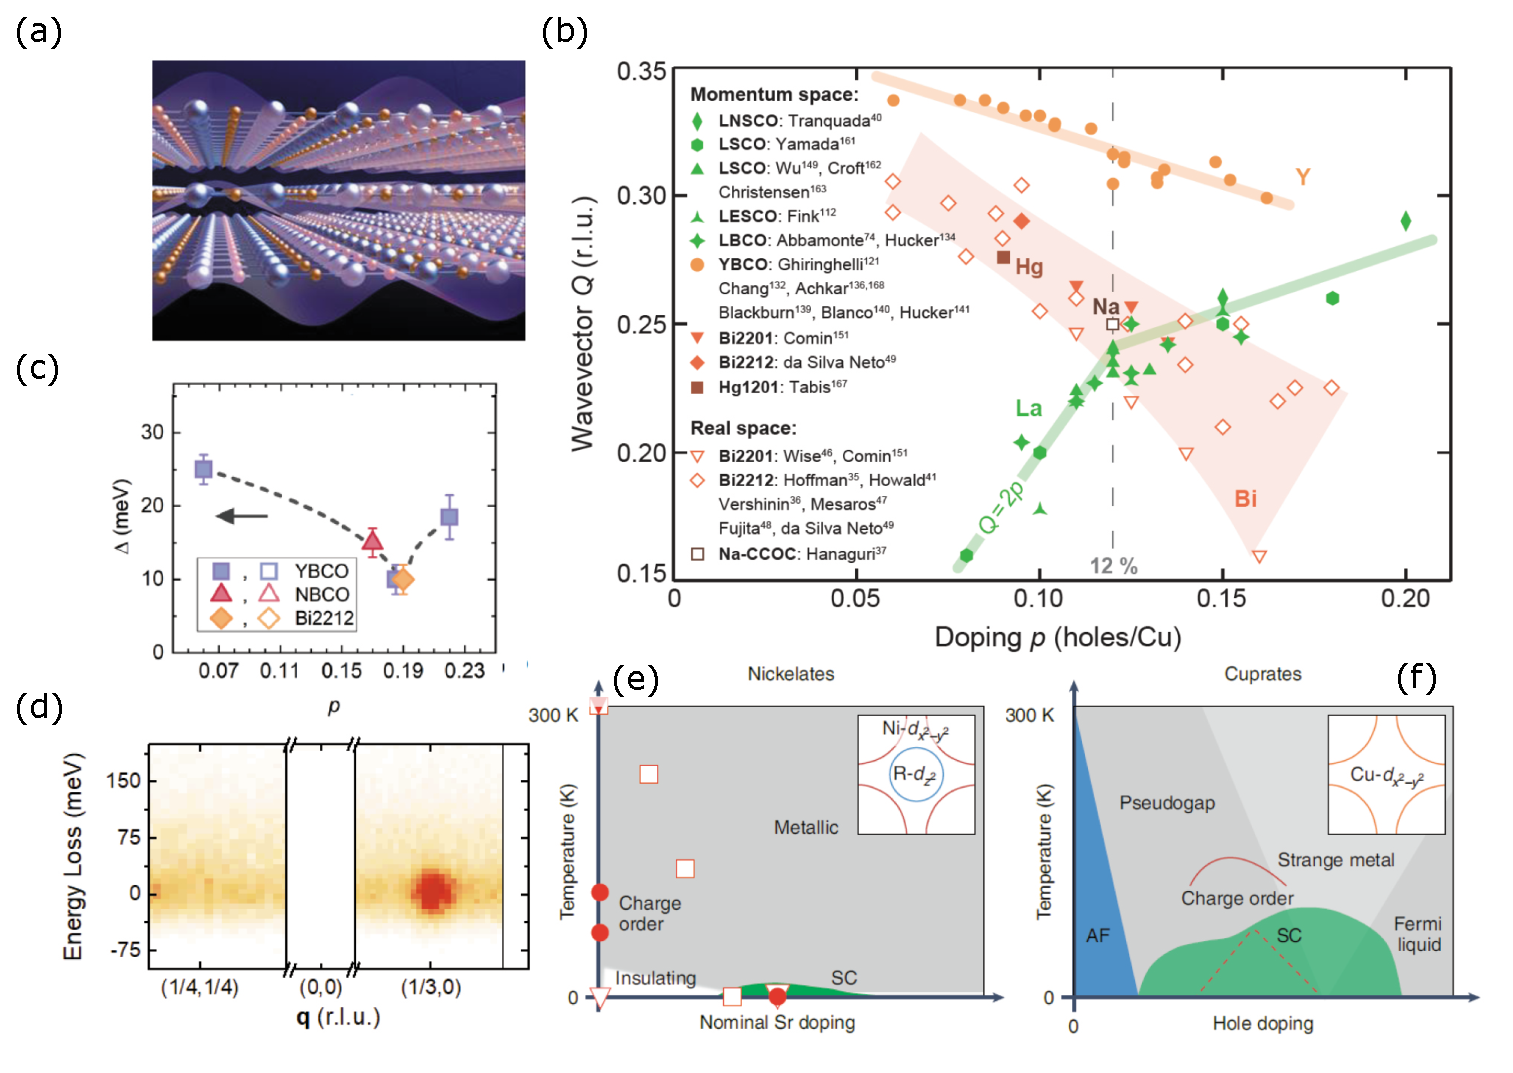
\includegraphics[width=0.99\textwidth]{cdw_tot2.eps}
    \caption{(a): pictorial representation of CDW in cuprates/nickelates (from Ref.~\cite{wahlberg2021restored}). (b): review of wavevector in different cuprate families as a function of doping (from \cite{comin2016resonant}). (c) energy of charge correlation with doping, showing a link to the Quantum critical point at $p=0.19$ (from Ref.~\cite{arpaia2022signature}). (d): first observation of CDW in nickelates (from my Ph.D.~thesis). (e)-(f): comparison of $T$-$p$ phase diagram in cuprates and nickelates (from \cite{benckiser2022neighbours}).}
    \label{fig:cdw}
\end{figure}
%
Interwoven with the anomalous normal state ($T>T_c$) properties of these materials are different types of broken translational and rotational symmetries, which involve either the charge, spin, or orbital degrees of freedom \cite{keimer2015quantum}.
Among them, the one which draws more attention are charge density waves (CDW), a modulation of the valence charge which is usually incommensurate with respect to the underlying lattice \cite{comin2016resonant}, and also spontaneously breaks its rotational symmetry (see e.g. the sketch in Fig. \ref{fig:cdw}\textcolor{blue}{a}). Their importance is especially evident in the family of cuprates, where they are universally present \cite{comin2016resonant} in a large portion of the temperature-doping ($T$-$p$) phase diagram.
At present, it is still unknown whether CDW originate from an instability of the lattice itself (phonon-driven scenario \cite{wang2021charge}) or from the structure of the Fermi surface \cite{comin2014charge}. Moreover, a recent work that I co-authored during my PhD studies shows that charge correlation might be linked with the putative Quantum Critical Point at doping $p\sim0.19$ \cite{arpaia2022signature}: indeed, as shown in panel (c) of Fig.~\ref{fig:cdw}, the energy of charge correlations reaches a minimum at the critical doping.
While the formation of charge stripes is a common result of the Hubbard model, even the more sophisticated calculations fail to reproduce the ensemble of experimental observations, even on a qualitative point of view \cite{comin2014charge, jiang2019superconductivity, marino2022stripes}. In particular, the doping dependence of the charge-order wavevector exhibits stark differences between cuprate families \cite{comin2016resonant} (see. Fig.~\ref{fig:cdw}\textcolor{blue}{b}), which still remain unexplained. 

\medskip

The importance of CDW for the physics of strongly-correlated materials has even strengthened recently, with their discovery in the new class of nickelate superconductors \cite{li2019superconductivity}. The interest around this family of materials stems from the fact that they mimic the lattice and electronic structure of cuprates: NiO$_2$ planes, arranged in a square lattice, with Ni$^{1+}$ in a $3d^9$ state \cite{hepting2020electronic, been2021electronic}.
A few months ago, three independent works (one of which I authored \cite{krieger2022charge}) have reported a phase with broken translational symmetry \cite{krieger2022charge, rossi2022broken, tam2022charge}. The CDW peak measured in a NdNiO$_2$ is shown in Fig.~\ref{fig:cdw}\textcolor{blue}{d}.
These measurements have highlighted significant discrepancies between CDW in Nickel and Copper compounds. Doping and temperature dependence are, in particular, clearly different as shown in panels (e)-(f) of Fig.~\ref{fig:cdw}. These preliminary results also show a qualitative agreement, but strong quantitative differences between La$_{1-x}$Sr$_x$NiO$_2$ and Nd$_{1-x}$Sr$_x$NiO$_2$, suggesting that rare-earth bands might play an important role. The orbitl character of these correlations is also, at present, under intense debate \cite{krieger2022charge, tam2022charge}.
%Additionally, we note that a few weeks ago the presence of CDW in the Ruddlesden-Popper (RP) compound La$_4$Ni$_3$O$_8$ was reported. RP compounds are not structurally equivalent to infinite-layers, but can still host superconductivity. Suprisingly, 
Therefore, much more experimental work is required and foreseen, and this topic is likely to stimulate a great amount of fundamental research in the next years.

\medskip

%
\begin{figure}
    \centering
    \includegraphics[width=0.99\textwidth]{ML5.pdf}
    \caption{Denoising of diffraction data using a CNN. (a)-(c): two-dimensional images of high-count, low-count, and CCN-denoised images. (d)-(f): extracted one-dimensional scans along the vertical direction of the images, in the horizontal point indicated by the red circle in panel (g)-(h): exmaples of a low-count and high-count RIXS image, respectively. Panels (a)-(f) readapted from \cite{oppliger2022weak}; panels (g)-(h) are raw data from one of my experiments, whose data have been recently published \cite{martinelli2022fractional}.}
    \label{fig:ML}
\end{figure}
%
How to unravel the complexity of unconventional superconductors? While lab-based techniques are still widely employed, many fundamental results come from experiments performed at large-scale facilities such as neutron sources and synchrotrons. In the last years, neutron/x-ray diffraction, elastic and inelastic scattering, but also synchrotron-based photoemission have shaped our knowledge of strongly-correlated materials \cite{keimer2015quantum}. 
They have, for example, given access to the electronic structure, to the magnetic and orbital dynamics, and to the broken-symmetry phases of countless materials.

Many of these techniques, however, suffer from severe time limitations. Time allocated for experiments is usually very short (less than 6 days), and most of them require remarkably long acquisition times. As an example, a good-quality  Resonant Inelastic X-ray Scattering spectrum usually requires around an hour, and this time further increases when employing high-energy resolution, or when measuring thin films.
While many of these experimental techniques have benefited from huge advancements in instrumentation, improvements in data-collection algorithms have not kept the same pace. Most of these techniques employ two-dimensional pixel-sensitive detectors, so that collected data come in the form of images. Therefore, one option to improve their performance would be to apply modern deep-learning methods for image and curve denoising. Deep learning algorithms have made giant leaps in recent years in the field of image restoration \cite{zhang2017beyond, tian2020deep}, mostly thanks to the improvements in the design and training proedures of Convolutional-Neural-Networks. Many approaches have been developed, both in the form of supervised and unsupervised learning. Algorithms usually learn to denoise images by either training on pairs of noisy and ground-truth images \cite{zhang2017beyond, zhang2018FFDNet}, or pairs of noisy images (i.e. Noise-2-Noise \cite{lehtinen2018noise2noise}, Noise-as-clean \cite{xu2020noisy}), or even by cleverly using single images (Noise-2-Void \cite{Krull2019CVPR}, Noise-2-Self \cite{batson2019noise2self}).

%Moreover, algorithms can perform well on mixtures of Gaussian and Poisson noise, which are the relevant statistic describing typical experimental noise.

Application of these algorithms to physical measurements has been however very scarce, mostly applied to lab-based techniques such as Raman imaging \cite{valensise2020removing} or scanning probe microscopy \cite{borodinov2019deep}. One of the reason is that the effectiveness of denoising procedures depends on the accuracy of their assumptions on the structure of collected data. Therefore, the characteristics of the network have to be tailored and adapted to a precise technique. This requires an adequate knowledge of the structure of the data, of typical signals, and of the type of noise statistics.
The host group of Prof.~Chang has very recently pioneered the use of CNN for denoising of weak diffraction signals \cite{oppliger2022weak}. An example of the denoising procedure is reported in panels (a)-(f) of Fig.~\ref{fig:ML}. So far, however, such approaches were never applied to neutron and x-ray spectroscopies, such as (Resonant) Inelastic Neutron (INS) and X-ray Scattering (IXS/RIXS). 

\section{Planned research activities and schedule}

\subsection{Planned research activity}
Milestone (1) concerns the development and the training of CNN algorithms for RIXS denoising and will benefit from the expertise acquired by Prof.~Chang’s group \cite{oppliger2022weak}. First, it will be necessary to collect a suitable set of RIXS data. An efficient training requires a total number of pixels above $10^8$ \cite{oppliger2022weak}. RIXS images are composed of $2048\times2048$ pixels, but usually just half of them (in every direction) contain significant intensity. Therefore, considering a conservative number of ``useful'' pixels of $10^6$ per each frame, one needs around $\sim10^3$ RIXS images. This number is close to what is acquired in a single RIXS experiment, and a suitable dataset can be retrieved from the previous experiments performed by the group of Prof.~Chang. Previous works on denoising of other thecniques show that usually the best networks are those trained on pairs of low-counts and high-counts images \cite{oppliger2022weak}. 
Therefore, corresponding images will have to be aligned and summed to produce high-count frames (see e.g. panels (f) and (g) in Fig.~\ref{fig:ML}). 
However, other approaches that do not require ground truth pairs, such as noise-2-noise and noise-2-self, might produce good results. Since the topic is new, these will have to be explored as well.
Following \cite{oppliger2022weak}, we will first employ IRUNet CNN architecture \cite{irunet}; the number of layers, as well as the kernel size, will have to be optimized. 

\medskip

Projects (2) and (3) require the use of state-of-the-art synchrotron instrumentation.

Milestone (2) concerns the investigation of the correlation between stripe/charge order and phonons. In particular, we will study samples of La$_{2-x}$Sr$_x$CuO$_4$ (LSCO).  The investigation of charge-order is complicated by the presence of multiple domains in the CuO$_2$ plane, with perpendicular orientation of stripes (twinning). However, it was recently shown by diffraction measurements \cite{choi2022unveiling} that the application of a moderate uniaxial strain removes the twinning and pins stripes to a single direction. Therefore, we will make use of the strain cells developed and optimized by the group of Prof.~Chang \cite{wang2022uniaxial, choi2022unveiling}. A sketch of the device is shown in Fig.~\ref{fig:strain}, which also reports schematically the effect of strain on the position of CDW peaks. \\
% will be ideally carried out on two beamlines: I21 of Diamond Light Source for RIXS measurements, in collaboration with Dr.~Jaewon Choi, beamline scientist and former PostDoc of the host’s group, and ID28 of the European Synchrotron Radiation Facility, for the ultra-high resolution IXS measurements. 
Ideally, this project requires the use of two different techniques: RIXS and high-resolution IXS.
RIXS  measurements will be performed on beamline I21 of Diamond Light Source. We will first measure at Oxygen $K$-edge, where the energy resolution is higher. In particular, we will acquire RIXS spectra with a transferred momentum parallel and perpendicular to the charge modulation. 
Indeed, experiments on other cuprates show that detwined CDW lifts the degeneracy of phonons along the directions parallel and perpendicular to the stripes \cite{pint2004oxygen,reznik2003oxygen}. We will precisely determine the energy, width and intensity of the high-energy branches, discriminating between those affected and insensitive to stripe formation. 
This will allows us to identify anomalies in the phonon self-energy \cite{wang2021charge, dashwood2021probing} but also in the electron-phonon coupling, exploiting its direct relation with RIXS intensity \cite{braicovich2020determining}. 
%
\begin{wrapfigure}{r}{0.35\textwidth}
  \centering
    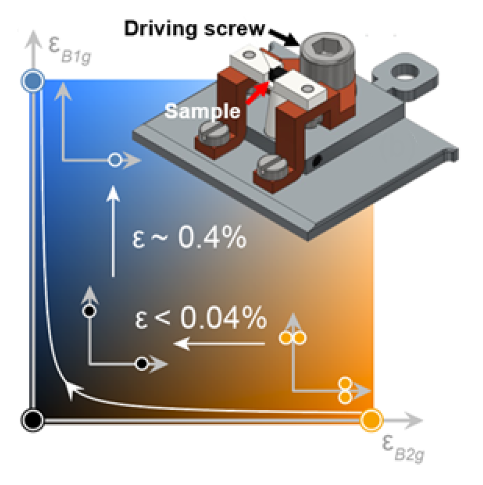
\includegraphics[width=0.3\textwidth]{straincell.eps}
  \caption{Sketch of the strain cell for the application of uniaxial strain developed in the group of Prof.~Chang. Colored maps shows the result of applications of $B_{1g}$ uniaxial strain along Cu-O bonds (vertical axis), which detwins charge-order. Small cartesian axes display the position of CDW peaks in reciprical space. Adapted from \cite{wang2022uniaxial}.}
  \label{fig:strain}
\end{wrapfigure}
%
Therefore, we will carefully quantify how high-energy phonons are affected by (or correlated with) the onset of the CDW order.
We will complement RIXS measurements with high-resolution Inelastic Scattering Scattering (IXS), to be performed on beamline ID28 of the ESRF. IXS is not directly sensitive to the electron-phonon coupling, but possess a much higher energy resolution than RIXS. Therefore, we will be able to track the evolution of low-energy phonons across the onset of stripe order. We note that a similar study was performed on other cuprates \cite{le2014inelastic}, where the phenomenology of charge order is different.

%Therefore, we will, for the first time, precisely determine how the high-energy phonon branches phonon branches are affected

Milestone (3) deals with diffraction measurements of charge-order in infinite-layer nickelates. Since this material can (at least at the moment) only realized in the form of very thin films ($\sim10\!$ nm thickness \cite{li2019superconductivity, krieger2022charge}), surface diffraction is the best choice. We will perform measurements at the beamline P07 at PETRA-III (DESY), whose sensitivity is more than appropriate to study 10 nm films \cite{albertin2020surface}. The goal will be to shed light on the properties of charge-order, which at the moment are still widely unknown. First, we will explore in detail the out-of-plane character of charge correlations, exploring the $c$-axis dependence of the structure factor across many Brillouin zones. Secondly, we will study in detail the temperature dependence of charge correlations, using the cryostat installed at the beamline.
Finally, we will also study how the characteristics of charge order are affected by the rare-earth atom, by studying both NdNiO$_2$ and PrNiO$_2$ thin films. Indeed, it has been extensively demonstrated that the rare-earth electronic bands are active at the Fermi level \cite{hepting2020electronic, been2021electronic}.


We stress that results in milestone (1) will undoubtedly be extremely beneficial for the data analysis of projects (2) and (3). 


\subsection{Schedule}
The proposed research is planned to be part of a two-year Postdoc project, with the funded period beginning in September 2023. The three milestones in which it is structured are designed to be run in parallel.
%Our research is structured into three milestones that can be addressed in parallel.

Each of them has three phases: preparation, execution, and communication/publication. 
Project (1) requires some education on convolutional neural network (CNN) algorithms applied to image denoising developed by the group of Prof.~Chang. This training will benefit from my background in machine-learning techniques acquired during my graduate studies. This phase will be carried out during the evaluation of this application and will therefore be completed before the beginning of the funding period. 
The other two parts of the project (milestones 2 and 3) rely on synchrotron instrumentation that is accessed through the submission of beamtime proposals. The time between submission to actual scheduling of successful proposals involves a lead time of more than six months. 
Two experiments, whose proposals had been submitted during the last months, have already been accepted for the next round of beamtime. In particular, a RIXS experiment on the interplay of charge-order and phonons on La-based cuprates involving the use of strain cells has been granted beamtime at the I21 beamline of Diamond Light Source. At the same time, a surface diffraction experiment on infinite-layer nickelates has been scheduled for the summer on beamline P07 of PETRA III.
We will further submit additional beamtime proposals in the next months, during the evaluation phase of this grant. In this way, the execution phase will start immediately at the beginning of the funding period.

As a bullet-point overview, our project will progress as follows:

\begin{enumerate}
    \item March - September 2023 – At this time, education of sample preparation techniques needed for project (2) will be completed. Regarding Project 1, we will first identify and pre-process suitable datasets required to train the algorithm, as described in the previous section. Then, the development of the CNN algorithm will begin, using IRUNet developed for denoising of diffraction as a starting point. I expect to already obtain preliminary results on this milestone at the end of this phase.

    \item September 2023 -- March 2024 – Synchrotron experiments and further development of CCN algorithms. The work on the three milestones will proceed in parallel, since time allocated for synchrotron experiments does not exceed one week per approved experiment. Another round of beam-time proposals will be submitted to different synchrotron facilities (the submission deadlines are spread between the beginning of September and the middle of October). At the end of this period, results on project (1) are expected.

    \item March-July 2024 – Data analysis of first synchrotron experiments will be completed. Depending on the results that will be achieved, it might be interesting to complement them with theoretical calculations. They will likely require a few ($\sim3/4$) additional months. Depending on the results achieved, another round of proposals will be submitted at beginning of March. First submission to high impact journals regarding project (1) is expected. During this period, we will continue with synchrotron projects.

    \item Second-half of 2024 – I expect publication of the results obtain for milestone (1) during this period. At the same time, milestones (2) and (3) will come close to completion. Data analysis of the next-round of synchrotron experiments will be finished, so that I will start the writing and submission of related papers to physical journals.
    
\end{enumerate}

After completion of the research plan proposed in this project:

\begin{enumerate}[resume]
    \item First half of 2025 – Submission of the results in milestones (2) and (3) will be definitely completed. In the meantime, I job and grant applications aiming at an independent research position will be written and submitted. Grant and job interviews.

    \item 	Second half of 2025 – After the completion of the research project and the evaluation of the submitted applications, I expect to start my own independent research group at a university or national research facility.
\end{enumerate}

Common to scientific planning, this project is setup quite optimistic in terms of time scales. We are aware that setbacks or unpredictable limitations could possibly occur. To mitigate such risk factors, I have purposely designed the project with three milestones that can be pursued in parallel. I am therefore confident that the proposed activity will deliver results with high impact and immediate interest for the condensed matter physics community.

\section{Available resources}

This first milestone of this project involves the use of deep learning algorithms, and therefore requires the use of GPU time. The group of Prof.~Chang has a collaboration with Prof.~Nicola Serra, whose cluster was used to perform the training of the CNN used to denoise diffraction data \cite{oppliger2022weak}. Additionally, a large datasets of RIXS images is required (as described in the previous section). This is, however, already available thanks to the number of experiments performed by the group of Prof.~Chang in the recent years. 

The experimental activities of this project (milestone 2 and 3) require the use of synchrotron radiation and instrumentation, of high-quality samples, and computational resources for data analysis. 
Access to synchrotron beamlines is subject to the approval of proposals, which can be submitted in two different rounds every year. We can also benefit from the support of the beamline staff. They also require the use of cuprates and nickelates samples, which will have to be grown and characterized. Samples of LSCO will be provided by the group of Prof.~Tohru Kurosawa from Muroran Institute of Technology, whose high-quality samples have been already used by Prof.~Chang \cite{wang2021charge, wang2022uniaxial}. 
Infinite-layer nickelates samples will be provided by two different sources: the group of Prof.~Zhihai Zhu from Beijing National Laboratory for Condensed Matter Physics (China), who has already collaborated with Prof.~Chang \cite{gaoMagneticExcitationsStrained2022}, and the group of Daniele Preziosi at University of Strasbourg, with whom I have closely worked during my PhD studies \cite{krieger2022charge}.
The laboratories at the University of Zurich also possess the infrastructure required to perform some sample characterization: a SQUID magnetometer for magnetic susceptibility measurements, and a PPMS for resistivity measurements.
Data analysis of diffraction or x-ray inelastic scattering is not computationally demanding, and can be performed with a commercially available laptop, of which I am already in possession. Additionally, I already possess the skills required to efficiently extract and analyse synchrotron data thanks to my doctoral experience.


\section{Significance of the expected results of the project}
This project assesses issues and topics that are currently stimulating advanced and high-impact research. 
The development of a CNN for RIXS denoising will be the first attempt to use deep-learning approaches to enhance the performance of an x-ray spectroscopy. The field of machine learning is, at present, among the most prolific in science.
Overall, I expect that this pioneering study  will be deemed important by the synchrotron community, and will certainly stimulate further research. Indeed, many spectroscopies rely on the acquisition of two-dimensional images (e.g. time-of-flight neutron scattering). 
%Overall, I expect that research in this direction will be deemed important by the synchrotron community, and by the physics community in general, and be published in high-impact journals.
%Moreover, a first pioneering study in this direction will certainly stimulate further research. Indeed, many spectroscopies rely on the acquisition of two-dimensional images (e.g. time-of-flight neutron scattering).

The study of charge density waves and charge fluctuations in cuprates and nickelates is one of the most active areas of research in the field of strongly correlated materials. The different phenomenology of the charge-ordered phase displayed by the cuprates is fascinating, and at present still unexplained. Therefore, providing an answer to this question would certainly be a fundamental result in the physics of strongly-correlated materials. 
At the same time, the recent discovery of similar charge-ordering in infinite-layer nickelates has certainly strengthened its importance. The first studies have highlighted some interesting features, but are very incomplete. As an example, very little is yet known about the possible three-dimensional character, precise doping dependence, and eventual coupling to phonon branches. Due to the interest in the topic, I expect that our results will be appreciated by the physics community, and will find publication in important physical journals.

\medskip 

With regard to my personal development, I believe that carrying out a PostDoc at the University of Zürich in the group led by Prof.~Johan Chang is a great opportunity for my scientific career. 
The project presented here is ambitious. 
The experimental activity will proceed in parallel, and ideally benefit from, a more technical advancement of the experimental technique itself.
It will give me the chance to acquire new skills and greatly expand my knowledge of experimental physics. 
I believe that the group of Prof.~Chang is the ideal place to conduct this project. 
Over the years, they have addressed complex  scientific cases in original ways, accompanying this more fundamental research with the development of novel scientific instruments.
Conducting a PostDoc in such a stimulating and high-profile environment will help me in reaching the independence required to become a leading researcher myself.
Indeed, after the completion of my PostDoc at the University of Zürich, my goal is to start my own research group at a physics department or in a research facility. 
I strongly believe that the experience and knowledge acquired during this project, combined with my doctoral education, will give me an important edge over the rest of the community. 



\nocite{apsrev41Control}    %needed for the paper titles
\bibliography{bibfile, revtex-custom}


\end{document}
